\documentclass[11pt,a4paper]{article} %title page
\usepackage[margin = 2cm]{geometry}


\usepackage{titletoc}
\usepackage[pagestyles]{titlesec}
\usepackage[no-math]{fontspec} 

%加這個就可以設定字體
\usepackage[CJKnumber, CJKchecksingle]{xeCJK} 
\usepackage[usenames,dvipsnames,svgnames,table]{xcolor}

\usepackage{paralist} % enhanced list environment
\usepackage{textcomp} % for including symbols
\usepackage{multicol} 
\usepackage{multirow}
\usepackage{threeparttable} %add footnote under tables
\usepackage{booktabs, tabularx} %extend control of width of columns 
%\usepackage{warpcol}%for decimal points alignment in tables


% packages about math
\usepackage{amssymb, amsmath, mathcomp} 

%for figs
\usepackage{placeins} % to flush all the floats before
\usepackage{graphicx}
\usepackage{wrapfig} %控制圖繞文 
\usepackage{float} % controlling the place of figure
\restylefloat{figure}

% for caption
\usepackage{caption, subcaption}
\usepackage{hyperref}

% for Reference
\usepackage[square, numbers, sort&compress]{natbib}
\usepackage[page,titletoc]{appendix} %toc for Appendices


%讓中英文字體分開設置
%設定中文的字型,可以直接輸入系統裡有的字型
\setCJKmainfont[BoldFont=DFHei Std W7]{DFHei Std W5}
\newCJKfontfamily{\kai}[BoldFont=DFKaiShu Std W7]{DFBiaoKaiShu Std W5}
\setmonofont[Mapping=tex-text]{Inconsolata}
%\setromanfont[Mapping=tex-text,BoldFont=Adobe Caslon Pro Bold]{Adobe Caslon Pro}
\setromanfont[Mapping=tex-text,BoldFont=Adobe Garamond Pro Bold]{Adobe Garamond Pro}
\setsansfont[Mapping=tex-text]{FuturaStd-Medium}
\newfontfamily{\optima}{OptimaLTStd}

\XeTeXlinebreaklocale "zh"
\XeTeXlinebreakskip = 0pt plus 1pt
%上面這二行,中文才能自動換行

\newcommand{\horrule}[1]{\rule{\linewidth}{#1}} 	% Horizontal rule
\newcommand{\nonumsubsec}[1]{\phantomsection \addcontentsline{toc}{subsection}{#1} \subsection*{\optima #1}}

\renewcommand{\thesection}{\Roman{section}}
\titleformat{\section}{\Large\bfseries}{\thesection.}{0.5em}{}
\renewcommand\figurename{圖}
\renewcommand\tablename{表}
%\renewcommand\lstlistlistingname{List of Source Codes}
%\renewcommand\lstlistingname{Code}


\newpagestyle{main}{\sethead{\small\kai\optima\sectiontitle}{\optima 2013 ML Final Project}{} \setfoot{}{\optima\thepage}{}\headrule}
%\newpagestyle{main}{\sethead{}{}{} \setfoot{}{\thepage}{}}

\renewcommand{\today}{\number\year 年 \number\month 月 \number\day 日}

%% Short-keys for easy typing
\newcommand{\figref}[1]{圖~\ref{#1}}
\newcommand{\tabref}[1]{表~\ref{#1}}

\newcommand{\scfi}[2] {\ensuremath{#1 \times 10^{#2}}}
\renewcommand{\t}[1]{\text{#1}}
\newcommand{\tk}{\text{k}}\newcommand{\tm}{\text{m}}
\newcommand{\tn}{\text{n}}\newcommand{\tM}{\text{M}}

\newcommand{\insertfig}[4]{\begin{figure}[H]
	\begin{center}
	\includegraphics[width = #2\textwidth]{#1}
	\caption{#3}\label{#4}
	\end{center}\end{figure}}
\newcommand{\insertfigx}[5]{\begin{figure}[#5]
	\begin{center}
	\includegraphics[width = #2\textwidth]{#1}
	\caption{#3}\label{#4}
	\end{center}\end{figure}}

\newcommand{\inserttable}[1]{
	\begin{table}[H]\vspace{-5pt}\begin{center}
	\input{#1}\vspace{-10pt}\end{center}\end{table}\vspace{-10pt}}
\newcommand{\inserttablex}[3]{
	\begin{table}[H]\begin{center}\caption{#2}\vspace{-10pt}\label{#3}
	\input{#1}\end{center}\vspace{-10pt}\end{table}}

%% end short-keys
\newcommand{\link}[2]{ \href{#1}{\textcolor{Gray}{#2}}}
\newcommand{\statatab}[1]{
\begin{table}[H]\centering\begin{threeparttable}
\input{#1}\end{threeparttable}\end{table}}

\usepackage{enumitem}

\pagestyle{main}
\begin{document}
%\setlength{\parindent}{0cm}
\setlength{\baselineskip}{1.5em}
\setlength{\parskip}{0.5em}

%%%%%% 抬頭 %%%%%%
\thispagestyle{empty}
\begin{center}
{\optima\LARGE Machine Learning Final Project}\\[0.5em]
電機五~王亮博~B98901114 \\
經研二~顏嘉儀~R01323019
\end{center}

%%%%% Workflow %%%%%%
\section{整理流程簡介}
基本上我們這組主要專注在 feature 的轉換與選擇,一開始的想法是想透過選出比較有意義的 feature,這樣也許用簡單的 model,例如 linear regression 就可以獲得不錯的準確度。很可惜的是從結果來說我們目前用的幾個方法都並沒有非常顯著的改善。在最後也會提出我們的推論,以及未來可以改進的方向。

\figref{fig:workflow-overview} 所示即為本次整體的處理流程,能分成 Feature Selection 以及 Model Selection 兩大部份。透過 feature selection 之後,我們可以得到不同種方法產生的多個 feature space。之後在 Train model 時,就可以從這些 feature 中選出一部份來 train 我們的 model。

由於我們選用的 feature 可能會牽涉到高維度的轉換, $v_{dc}$ 的增加會讓我們有 overfitting 的問題,所以我們對此有兩個可以解決的方向:
在 model 選擇上,我們會盡量選擇 $v_{dc}$ 較低的演算法,例如 SVM、有 regularization 的 regression。其次為盡量減少最後選用 feature 的數目,可以考慮用 PCA 等方向降維。比較可惜的是,因為時間的關係,我們還沒有做到減少 feature 選用;此外,我們在 feature 轉換中,「Bag-of-Words」的方法尚未實作出,會在下文繼續做相關的說明。

而在 Model Selection 的部份,SVM 類我們使用 cross validation 的方式,找出最佳的參數組合;在 Neural Network (NN) 設計我們同樣使用 cross validation 來去判斷如何調整我們 NN 的層數、node 數等。最後,我們比較這些 model 中找出一個在 validation 中表現最好重新以全部的資料 train,並上傳結果。

\insertfigx{workflow/overview}{0.4}{整體處理流程}{fig:workflow-overview}{htb}

以下便會針對 Feature Selection、Model Selection 作介紹,而實際在運作的過程中,我們也是將這兩部份拆開,分別完成。

%%%%%% Feature Selection %%%%%%%
\section{Feature Selection}
所有的操作皆在 Python 2.7/3.3 上進行。數值矩陣計算使用 Numpy 1.7+,而 SIFT 等跟影像計算有關的函式主要仰賴 OpenCV 2.4+/3.0-dev 版本,繪圖使用 matplotlib。

%%% FIG: Pixel view (raw and 60x60) %%%
\begin{figure}[htb]
    \centering
    \begin{subfigure}[b]{0.48\textwidth}
        \centering
        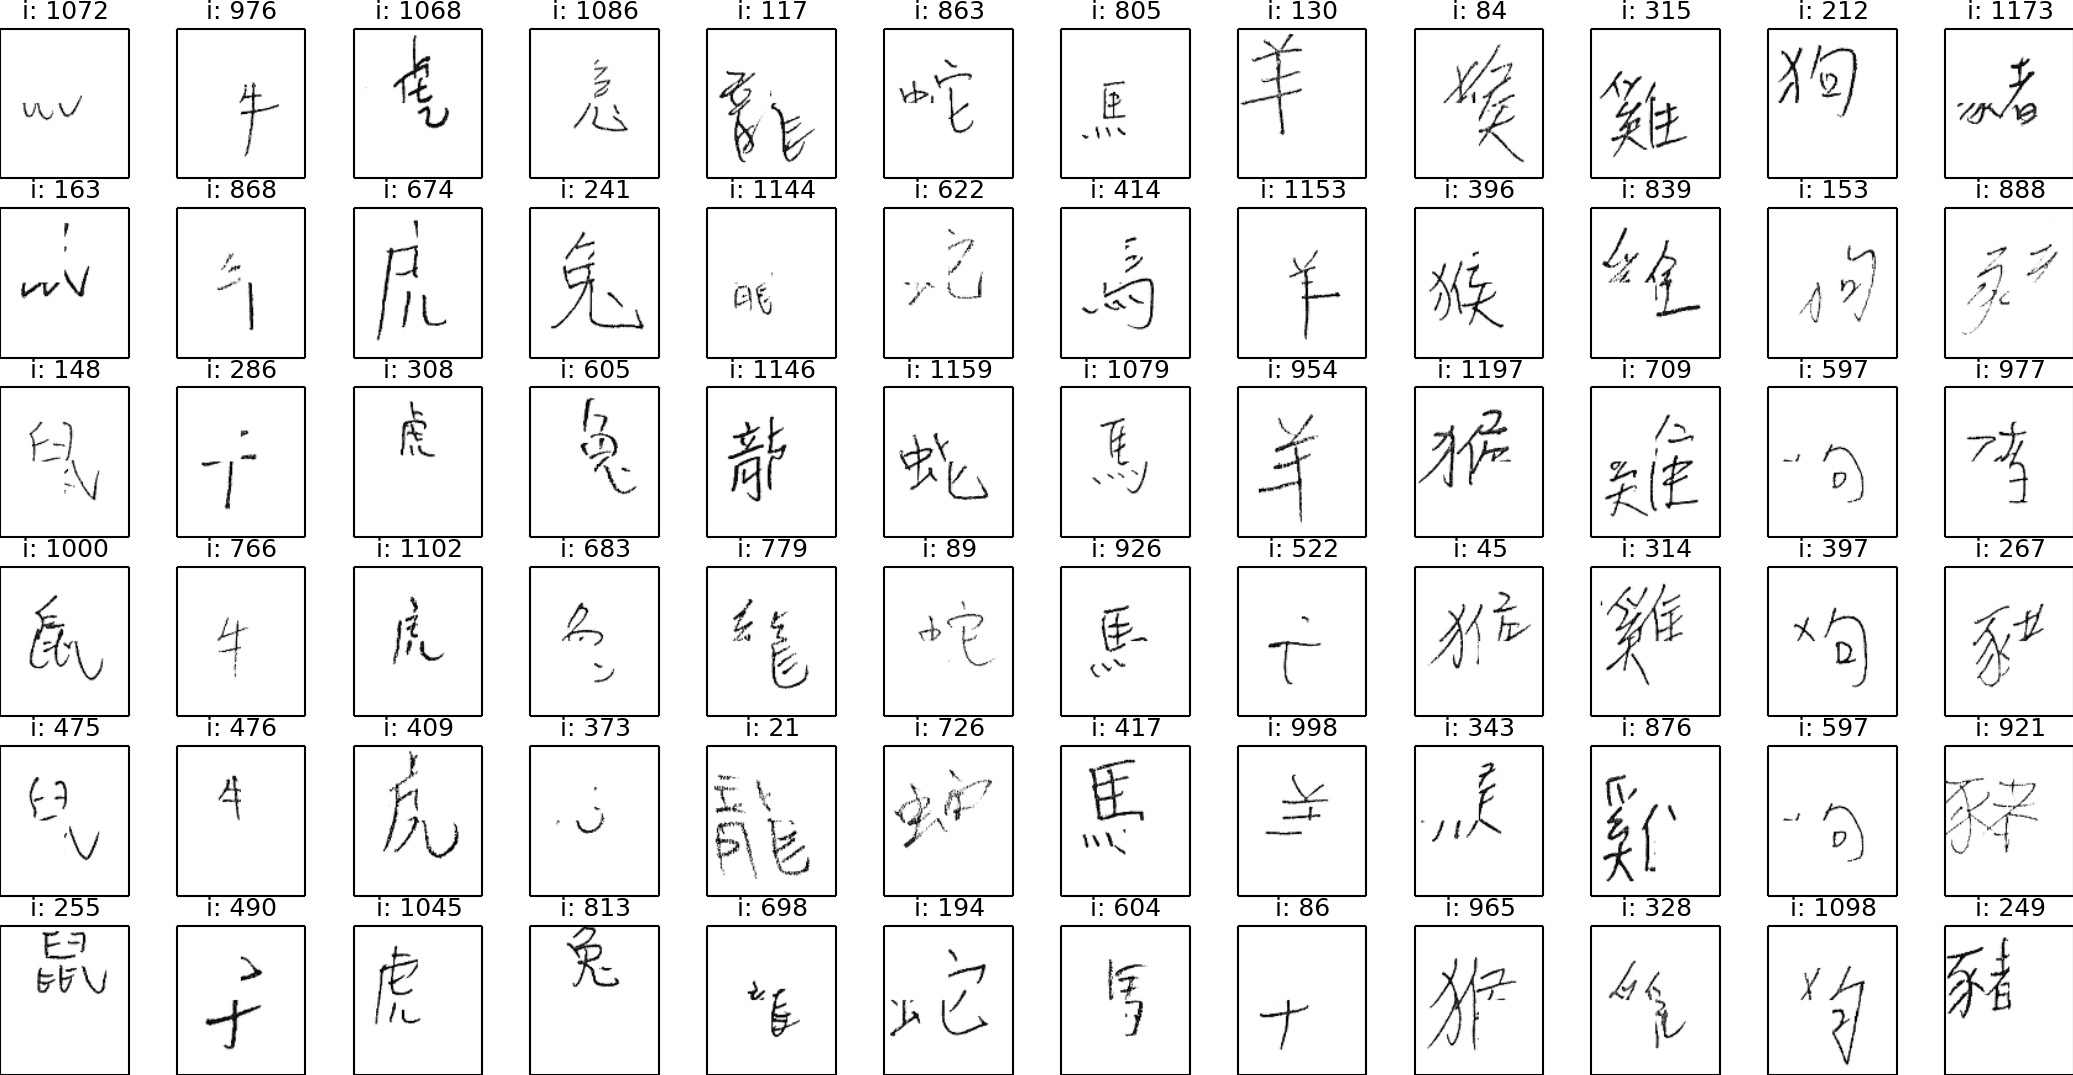
\includegraphics[scale=0.23]{../results/figs/train_pixelview_combined_6}
        \caption{Raw pixel input}
        \label{fig:px-raw}
    \end{subfigure}%
    ~
    \begin{subfigure}[b]{0.48\textwidth}
        \centering
        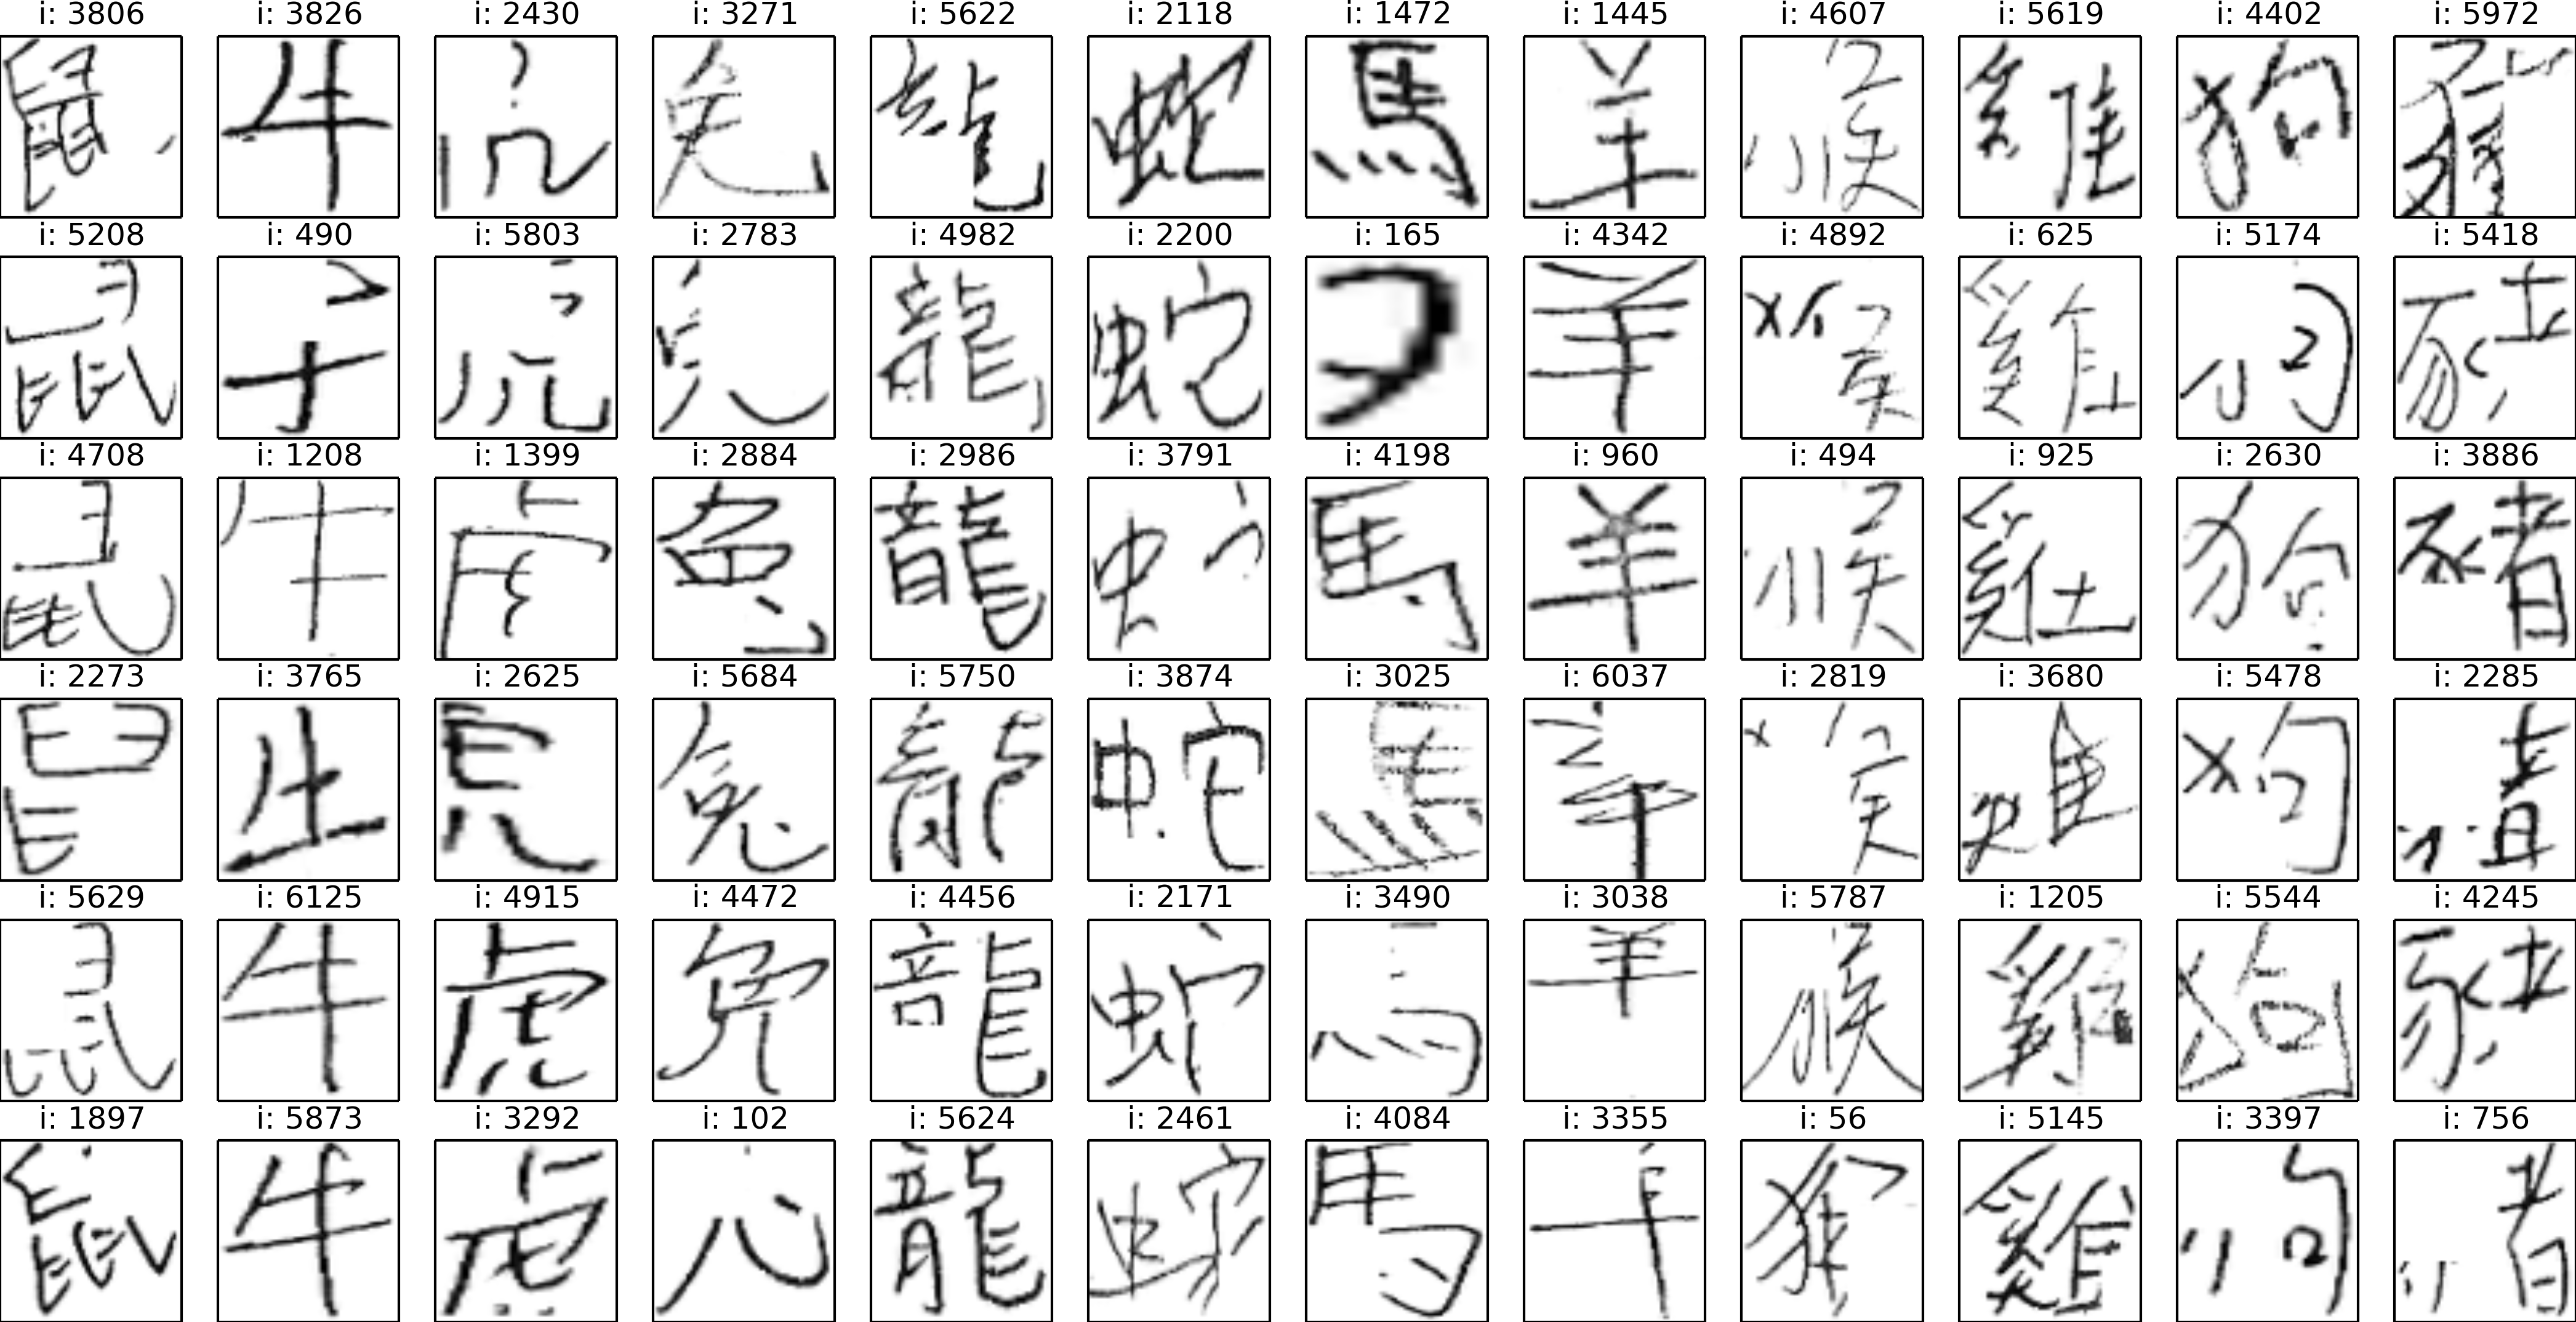
\includegraphics[scale=0.23]{../results/figs/train_pixelview_allzoidac_60x60_6}
        \caption{After 60x60 resize}
        \label{fig:px-60}
    \end{subfigure}
    \begin{subfigure}[b]{0.98\textwidth}
        \centering
        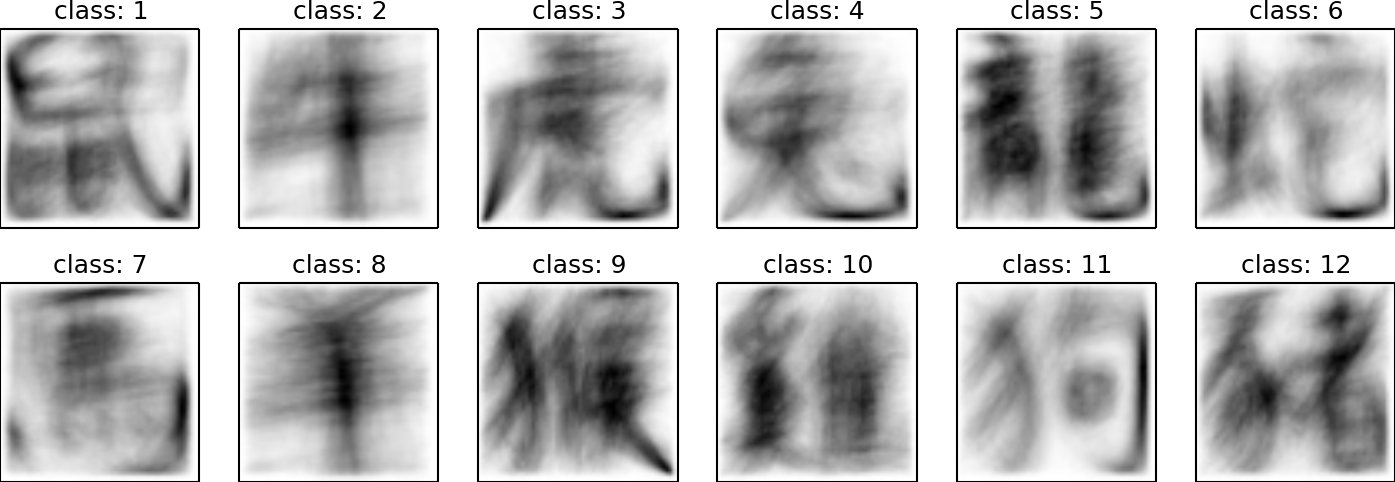
\includegraphics[scale=0.6]{../results/figs/60x60_avg}
        \caption{Aggregate mean of 60x60 resize data}
        \label{fig:px-60-mean}
    \end{subfigure}
    \caption{與 pixel 相關的 feature 概覽圖(可放大瀏覽)}\label{fig:px-overview}
\end{figure}

\subsection*{60x60 Resize}
首先應該預覽一下 data 的樣貌,可見\figref{fig:px-raw},發現每個字出現在的位置並非一致,故如果直接將這 12,810 個 feature 去 train model 表現將不理想,而我們實証結果也無法達到 50\% 以上的準確率。同時,由於 feature size 非常地大,但其實很多地方都是「空」的,一個字只佔用約 300 pixels 左右。因此我們第一個想解決的問題即是縮小 feature size,並且想辦法讓每個字都能大約在一樣的位置上,如此就能讓一個 pixel 的亮暗在整體上更具有意義,並且也能提昇計算速度。

所以我們選擇將原圖 resize 長寬皆 60 pixels,並且設定一個 threshold 將多餘的白邊的去除。60 僅是較原圖長寬小的尺寸,同時如果是跑 Linear SVM 的話,每一次 train 可以在 5 分鐘內完成,故我們覺得這個大小合理便一直沿用下去,resize 結果可見 \figref{fig:px-60}。參考 165(馬)、3038(羊) 等資料,因為在本來資料就有 1/4 遺失,resize 前者失去原有的空間特性(應該只是一個小小的勾),後者則是並沒有正確的將白邊去除。

當時初步認為這些資料處於「較少數之例子」,故我們傾向直接忽視他們。對於這些特例,前者可以藉由 resize 的比例來設定一個上限值,這樣以勾為例,就不會與正常馬的勾大小差距過多;後者則可以藉由二維的 histogram 來判斷畫素的分布是否跟該類別其他 data 差距明顯,或者利用一個 threshold 較大的白邊去除器,如果畫素分布不均,但在本例用另一白邊去除器時四邊切除之寬度差距會不等。

不過如果將轉換後的圖相疊做平均,見\figref{fig:px-60-mean},12生肖的字樣都能很清楚的浮現,這已較 raw 表現好,也達到起初目標。利用這樣的 feature 使用 RBF SVM 可以達到 7 成以上的準確度。這同時給了我們另一方向,因為往後考慮跟圖形特徵值辨識有關,在 raw 都有缺失資料的情況我們猜想即使是同組資料可能會有很不一樣的特徵值(例:剛好代表兩圖各缺失的角落),想要藉由將資料加上平均值來進行 model training,但以結論而言,由於 test data 並沒有這樣的特性,而在特徵值選取,由於平均值後,筆畫的邊界不是很明顯,即便使用 OpenCV 中 Adaptive Threshold 方式抓出邊界,預測效果不理想,故最後放棄了這條方法。

\subsection*{SIFT 演算法(Scale Invariant Feature Transform)簡介}
1999年, D.G.Lowe 提出SIFT 演算法\footnote{詳見``Object Recognition from Local Scale-Invariant Features'' (1999) 、``Distinctive Image Features from Scale-Invariant Keypoints'' (2004)},主要用來處理影像的旋轉、放大縮小、亮度變化、視角變換。舉例來說,當我們說某人長得很有特色時(像是蒜頭鼻?),我們已經抓到這個人的特徵了,之後不管這個人換怎髮型、服裝,我們都不會認錯那隻蒜頭鼻。同理,影像也是,只要我們能找到影像的關鍵特徵,那即使這張圖放大縮小、旋轉,我們都可以認得他。

那接著問題就變成,該怎麼找到影像得關鍵向量。關於這個問題,SIFT 提供一個解法,那就是 DOG 算子,



一旦有了每張圖的特徵向量,我們可以將兩張圖校正回同一個方向,並按照向量的長短,調整兩張圖到同樣大小,如上圖。套用到這次的資料,每個人寫的字大小且角度不一,藉由藉由 SIFT的幫助,有望反向校正回來。

\insertfigx{../results/figs/train_sift_allzoidac_60x60_}{0.9}{SIFT 特徵點標示示意圖。圖中每個圓圈皆為一個特徵點,橫線表該特徵點所代表之 patch gradient 方向,半徑大小與 $\sigma$ 有關,但實際 patch 較圓圈略大。}{fig:sift-result}{htb}


\subsection*{SIFT Datawise Pair Match}
這邊先對相關術語進行定義。每一筆資料 $i$,分別可能屬於 $Z=1,\ldots,12$ 生肖之一,$z$ 生肖擁有之總資料筆數定為 $I_z$。每筆資料 $i$ 經過 SIFT 後共有 $w_i$ 個特徵點 (visual word, VW),其第 $j$ 個特徵點對應之 gradient (descriptor) 為 $d_{i, j}$。任兩個 VW 可以利用 $M(w_a, w_b)$ 來計算出 距離(相似度),距離越短表示兩 VW 越像。

\subsection*{SIFT BoW Cluster}

\section{Model Selection}
\subsection*{Neural Network}

\insertfigx{../report/workflow/NN_overview}{0.6}{Back-propagation Neural Network}{fig:NN-overview}{htb}

類神經網路和模糊理論一直是電腦視覺的領域裡的資優生,在指紋識別、衛星影像分析有很好的成績。因此當我們拿到這次的資料,很自然的就會想試試看類神經網路。類神經網路與其他模型相比,有許多優點:
\begin{enumerate}[itemsep=-1ex]
\item 良好的推廣能力(generalization) :對於未知的輸入也可以得到正確的輸出。
\item 可處理雜訊:對一個訓練好的網路而言,即使輸入有些缺值,依然有能力正確辨識。
\item 分散式結構,不易損壞:即使部份神經元損壞,整體仍然可以正常工作。
\item 可以很輕易的導入非線性模型。
\end{enumerate}
其中特點 1、2、3 相當讓人興奮,因為這正好呼應著我們這次的資料:每張圖片都有 1/4 的缺值。

我們決定從倒傳遞網路出發(Back-propagation Network),模型設定如\figref{fig:NN-overview}。倒傳遞網路最讓人困擾的就是參數設定,像是:隱藏層數量、神經元數量、訓練函數、次數、學習速率等。針對這個問題,我們採用『閃開!讓專業的來』策略,參考文獻以縮小參數範圍。

\begin{enumerate}[itemsep=-0.5ex, topsep=0ex]
\item 隱藏層數量:

根據 Villiers and Barnard (2002),設在 1~2 層之間有較好的收斂效果,多於兩層不利收斂且容易掉入局部最小值,不但耗時又招致較大誤差。我們實作發現,兩層效果較好。

\item 神經元數量:

根據 Piroska and Zaletnyik (1999),當樣本數足夠大時,選擇  35 個神經元即可有效描述輸入輸出關係,但仍需視樣本大小、耗費時間而定。我們選擇以試誤法決定數目。

\item 學習速率與慣性項:

過大的學習速率不利收斂,易導致震盪 ; 過小的學習速率則是收斂變慢,計算耗時。參考 Andrew Ng 的線上課程,我們決定使用較小的 learning rate,避免錯過最佳解。同時配合較大的慣性項,以避免落入局部最小值。最後我們決定學習速率設為設為 0.005,慣性設為 0.9。

\item  訓練次數、訓練比例:

參考 Stack Overflow 大大們的討論,通常訓練次數設在200左右,就有不錯的表現,太多則容易導致過度配適。關於 validation set 的比例,大大們提醒了一件事:確保你的 training set 具有足夠的代表性!更白話一點,小心拔掉的  validation set 使得  training set 改變分佈。從善如流,我們設定200次訓練、10\% validation set。

\item 樣本數與其他:

在訓練過程中,我們發現使用 6000 筆樣本進行訓練的結果,預測能力僅一成,幾乎等於亂猜。推測可能是樣本全開的  noise 量太多,反而學得不好。我們實驗性的使用小樣本,發現 600 個樣本點就有五成的預測力。最後,bias 項一定要記得打開,否則模型絕對不會收斂 !
\end{enumerate}
下表為部份實驗數據:

\begin{table}[htb]
\centering
\begin{threeparttable}
    \begin{tabular}{lrrrrrrrrr}
        \toprule
        no.&   sample&   Epoch&    學習速率&    慣性&   N1&   N2&       耗時&   Ein&  Eval\\
        \midrule
        1&     6144&    1000&   0.005&   0.9&   10&   10&   4h8m34s&   0.70&   0.88\\
        2&      615&    1000&   0.005&   0.9&   10&   10&    15m05s&   0.08&   0.43\\
        3&      615&     200&   0.005&   0.9&   10&   10&    14m07s&   0.07&   0.45\\
        3&      615&     200&   0.005&   0.9&   20&   20&    40m37s&   0.13&   0.51\\
        \bottomrule
    \end{tabular}
\end{threeparttable}
\end{table}

在簡單的設定下,類神經網路就顯著易於亂猜。但經過初步的嘗試後,我們發現類神經網路的缺點:
\begin{enumerate}[itemsep=-1ex, topsep=0ex]
\item 計算量非常大,訓練時間很長。
\item 對資料敏感,抽樣時要注意分佈有無平均。
\item 黑盒子,無法看出什麼是關鍵因子。
\item 參數的選擇無窮無盡,曠日耗時。
\end{enumerate}
缺點 1 與缺點 4 在硬體資源與訓練時間的壓力下,讓調整參數以獲得更好模型的方法,難以進行。我們決定將主力放在SVM的訓練上。

\subsection*{SVM}


\section{Performance Comparison}

\section{Conclusion}

\end{document}
